% Reporte de la Actividad 10
% Problemas clasicos de sincronizacion
\documentclass[12pt,oneside]{template/liverpoolthesis}
% !TEX root = ../Practica1_Hernandez_Andrea_Espino_Heriberto.tex
\usepackage[discipline=computer-science]{template/liverpoolthesis}
\usepackage[utf8]{inputenc}
\usepackage[T1]{fontenc}
\usepackage[spanish,es-nodecimaldot]{babel}

% Las referencias internas y las citas usan el mismo azul que los títulos.
\hypersetup{
  linkcolor = LiverpoolBlue,
  citecolor = LiverpoolBlue,
  urlcolor = LiverpoolBlue
}

% La marca de cada capítulo aparece en el encabezado, arriba de la regla.
\addto\captionsspanish{\renewcommand{\chaptername}{Ejercicio}}
\providecommand{\figureautorefname}{Figura}
\addto\captionsspanish{\renewcommand{\figureautorefname}{Figura}}

\graphicspath{{figuras/}}
\setlength{\headheight}{28pt}

% Inserta una captura de código y/o de ejecución.
% El tercer argumento es la etiqueta; el argumento opcional controla la altura.
\newcommand{\incluirevidencia}[4][0.70\textheight]{%
  \begin{figure}[H]
    \centering
    \includegraphics[
      width=0.95\textwidth,
      height=#1,
      keepaspectratio
    ]{#2}
    \caption{#3}
    \label{#4}
  \end{figure}%
}

% ---------- Datos de la portada ----------
\title{Práctica de laboratorio 1: Creación de procesos e hilos en C y Java}
\author{%
  Heriberto Espino Montelongo\\
  ID: 175199\\[1em]
  Andrea Hernandez Huerta\\
  ID: 175523\\[1em]
  \text{Profesor:} Dr. Victor Giovanni Morales Murillo}
\faculty{Universidad de las Américas Puebla (UDLAP)}
\school{Licenciatura en Ciencia de Datos}
\degree{Curso: Programación Concurrente}
\date{Fecha de entrega: \today}
\subject{Creación y ejecución de procesos e hilos en C y Java}


\title{Actividad 10: Problemas clásicos de sincronización}
\author{%
  Andrea Hernandez Huerta\\
  ID: 175523\\[1em]
  Heriberto Espino Montelongo\\
  ID: 175199\\[1em]
  \text{Profesor:} Dr. Victor Giovanni Morales Murillo}
\faculty{Universidad de las Américas Puebla (UDLAP)}
\school{Licenciatura en Ciencia de Datos}
\degree{Curso: Programación Concurrente}
\date{Fecha de entrega: \today}
\subject{Problemas productor-consumidor y lectores-escritores}

\addto\captionsspanish{\renewcommand{\chaptername}{Parte}}
\providecommand{\figureautorefname}{Figura}
\addto\captionsspanish{\renewcommand{\figureautorefname}{Figura}}

\begin{document}

\frontmatter
\maketitle
\tableofcontents
\listoffigures
\listoftables

\mainmatter

\chapter{Problema productor-consumidor}

\textbf{Instrucción.} Implementar un búfer circular compartido con capacidad
para cinco elementos. El programa debe incluir un hilo productor que genere y
deposite diez elementos, un hilo consumidor que retire y procese los diez
elementos, un semáforo binario \texttt{mutex}, un semáforo contador para los
espacios disponibles y otro para los elementos disponibles. Los índices
\texttt{inBuf} y \texttt{outBuf} deben controlar el arreglo circular. El
productor debe esperar si el búfer está lleno y el consumidor debe esperar si
está vacío.

\section{Entradas}

El programa utiliza un arreglo llamado \texttt{buffer} con cinco posiciones.
El productor genera los elementos del 1 al 10 y el consumidor retira esos
mismos diez elementos. Los dos hilos comparten el arreglo, los índices
\texttt{inBuf} y \texttt{outBuf}, y tres semáforos:

\begin{table}[H]
\centering
\caption{Datos iniciales del problema productor-consumidor.}
\label{tab:entradas-productor-consumidor}
\begin{tabularx}{\textwidth}{P{4.0cm} c L}
\toprule
\textbf{Elemento} & \textbf{Valor inicial} & \textbf{Función}\\
\midrule
\texttt{mutex} & 1 & Protege el acceso al búfer. Solo un hilo puede modificarlo a la vez.\\
\texttt{espacios} & 5 & Cuenta los lugares libres del búfer.\\
\texttt{elementos} & 0 & Cuenta los elementos disponibles para el consumidor.\\
\texttt{inBuf} y \texttt{outBuf} & 0 & Indican la posición donde se deposita o se retira el siguiente elemento.\\
\bottomrule
\end{tabularx}
\end{table}

Al inicio, el búfer está vacío. Por eso hay cinco espacios disponibles y no
hay elementos que el consumidor pueda retirar.

\section{Procesamiento}

El productor solicita primero un espacio mediante el semáforo
\texttt{espacios}. Después solicita \texttt{mutex} para entrar al búfer, deposita el elemento en
la posición \texttt{inBuf} y avanza el índice con la operación circular
\texttt{(inBuf + 1) \% 5}. Al terminar, libera \texttt{mutex} y aumenta el
semáforo \texttt{elementos}.

El consumidor realiza el proceso contrario. Primero solicita un elemento con
\texttt{elementos.acquire()} y después solicita \texttt{mutex}. Retira el
valor de la posición \texttt{outBuf}, avanza ese índice de forma circular,
libera \texttt{mutex} y aumenta \texttt{espacios}.

Los semáforos controlan dos situaciones distintas. \texttt{mutex} evita que
productor y consumidor modifiquen el arreglo al mismo tiempo. Los semáforos
\texttt{espacios} y \texttt{elementos} coordinan la condición del búfer: el
productor se bloquea cuando no hay espacio y el consumidor se bloquea cuando
no hay elementos.

\section{Prueba de escritorio}

La siguiente secuencia muestra una posible ejecución. Los valores de los
semáforos se escriben después de cada acción; durante la sección crítica,
\texttt{mutex} toma temporalmente el valor 0.

\begin{table}[H]
\centering
\caption{Prueba de escritorio del búfer circular.}
\label{tab:prueba-productor-consumidor}
\begin{tabularx}{\textwidth}{c L c c L}
\toprule
\textbf{Paso} & \textbf{Acción} & \textbf{Semáforos} & \textbf{Índices} & \textbf{Búfer y estado}\\
\midrule
0 & Estado inicial & 1/5/0 & 0/0 & [\_,\_,\_,\_,\_]. Ambos hilos están activos.\\
1 & Productor deposita 1 & 1/4/1 & 1/0 & [1,\_,\_,\_,\_]. El consumidor puede continuar.\\
2 & Productor deposita 2 & 1/3/2 & 2/0 & [1,2,\_,\_,\_].\\
3 & Productor deposita 3 & 1/2/3 & 3/0 & [1,2,3,\_,\_].\\
4 & Productor deposita 4 & 1/1/4 & 4/0 & [1,2,3,4,\_].\\
5 & Productor deposita 5 & 1/0/5 & 0/0 & [1,2,3,4,5]. El búfer está lleno.\\
6 & Productor intenta depositar 6 & 1/0/5 & 0/0 & El productor se bloquea al solicitar un espacio.\\
7 & Consumidor retira 1 & 1/1/4 & 0/1 & [\_,2,3,4,5]. Se libera un espacio y el productor puede continuar.\\
8 & Productor deposita 6 & 1/0/5 & 1/1 & [6,2,3,4,5].\\
9 & Consumidor retira 2 & 1/1/4 & 1/2 & [6,\_,3,4,5].\\
\bottomrule
\end{tabularx}
\end{table}

\section{Salidas y evidencia}

La captura muestra el código Java del productor-consumidor y varias
ejecuciones del programa. En cada ejecución aparecen diez mensajes del
productor y diez mensajes del consumidor. Los índices recorren las posiciones
de 0 a 4 y vuelven a 0, lo que comprueba que el arreglo se utiliza como un
búfer circular.

\incluirevidencia[0.72\textheight]
  {Captura de pantalla 2026-10-03 a la(s) 10.33.56 a.m..png}
  {Código Java y salidas del problema productor-consumidor.}
  {fig:productor-consumidor}

\section{Conceptos utilizados}

El \texttt{mutex} representa exclusión mutua porque solo permite que un hilo
entre al búfer a la vez. Los semáforos contadores realizan sincronización
condicional: el productor depende de que exista un espacio y el consumidor
depende de que exista un elemento. Por tanto, un hilo puede quedar bloqueado
sin que exista un error; se desbloquea cuando el otro hilo cambia el estado del
búfer.

\chapter{Problema lectores-escritores}

\textbf{Instrucción.} Implementar una base de datos sencilla representada
mediante una variable compartida. El programa debe incluir tres hilos
lectores, dos hilos escritores, la variable \texttt{numReaders}, el semáforo
binario \texttt{mutex} para protegerla y el semáforo binario \texttt{wlock}
para controlar el acceso a la base de datos. También debe incluir los métodos
\texttt{startRead()}, \texttt{endRead()}, \texttt{startWrite()} y
\texttt{endWrite()}. Varios lectores deben poder acceder simultáneamente, pero
cada escritor debe tener acceso exclusivo.

\section{Entradas}

La base de datos se representa con la variable \texttt{baseDatos}, que inicia
en 0. La variable \texttt{numReaders} cuenta los lectores que están dentro de
la sección de lectura. El programa crea tres lectores y dos escritores; los
escritores escriben los valores 100 y 200.

\begin{table}[H]
\centering
\caption{Datos iniciales del problema lectores-escritores.}
\label{tab:entradas-lectores-escritores}
\begin{tabularx}{\textwidth}{P{4.0cm} c L}
\toprule
\textbf{Elemento} & \textbf{Valor inicial} & \textbf{Función}\\
\midrule
\texttt{baseDatos} & 0 & Variable compartida que leen los lectores y modifican los escritores.\\
\texttt{numReaders} & 0 & Cuenta cuántos lectores están leyendo.\\
\texttt{mutex} & 1 & Protege el contador \texttt{numReaders}.\\
\texttt{wlock} & 1 & Permite el acceso exclusivo de los escritores y del grupo de lectores.\\
\bottomrule
\end{tabularx}
\end{table}

\section{Procesamiento}

Cuando un lector inicia, ejecuta \texttt{startRead()}. Primero solicita
\texttt{mutex} y aumenta \texttt{numReaders}. Si es el primer lector,
solicita también \texttt{wlock}; así evita que un escritor modifique la base
de datos mientras haya lectores. Después libera \texttt{mutex}. Los lectores
que llegan después pueden entrar porque \texttt{wlock} ya está ocupado por el
grupo de lectores.

Al terminar, cada lector ejecuta \texttt{endRead()}. Solicita \texttt{mutex},
disminuye \texttt{numReaders} y, si ya no queda ningún lector, libera
\texttt{wlock}. Finalmente libera \texttt{mutex}.

Un escritor ejecuta \texttt{startWrite()} para solicitar \texttt{wlock}.
Mientras lo tiene, ningún lector nuevo puede entrar y ningún otro escritor
puede modificar la base de datos. Después de escribir, ejecuta
\texttt{endWrite()} y libera \texttt{wlock}.

\section{Prueba de escritorio}

La siguiente secuencia muestra primero la entrada de los tres lectores y
después la entrada exclusiva de los dos escritores. Los valores de
\texttt{mutex} y \texttt{wlock} se muestran después de cada acción.

\begin{table}[H]
\centering
\caption{Prueba de escritorio del problema lectores-escritores.}
\label{tab:prueba-lectores-escritores}
\footnotesize
\renewcommand{\arraystretch}{1.05}
\begin{tabularx}{\textwidth}{c L c c L}
\toprule
\textbf{Paso} & \textbf{Acción} & \textbf{numReaders} & \textbf{mutex/wlock} & \textbf{Estado}\\
\midrule
0 & Estado inicial & 0 & 1/1 & Lectores y escritores disponibles.\\
1 & Lector 1 ejecuta \texttt{startRead()} & 1 & 1/0 & Lector 1 lee; los escritores quedan bloqueados.\\
2 & Lector 2 ejecuta \texttt{startRead()} & 2 & 1/0 & Lectores 1 y 2 leen al mismo tiempo.\\
3 & Lector 3 ejecuta \texttt{startRead()} & 3 & 1/0 & Tres lectores están activos.\\
4 & Lector 1 ejecuta \texttt{endRead()} & 2 & 1/0 & Lector 1 sale; los escritores siguen bloqueados.\\
5 & Lector 2 ejecuta \texttt{endRead()} & 1 & 1/0 & Lector 2 sale; Lector 3 continúa.\\
6 & Lector 3 ejecuta \texttt{endRead()} & 0 & 1/1 & Se libera \texttt{wlock}.\\
7 & Escritor 1 ejecuta \texttt{startWrite()} y escribe 100 & 0 & 1/0 & Escritor 1 tiene acceso exclusivo.\\
8 & Escritor 1 ejecuta \texttt{endWrite()} & 0 & 1/1 & La base de datos queda disponible.\\
9 & Escritor 2 escribe 200 y libera \texttt{wlock} & 0 & 1/1 & Escritor 2 también entra de forma exclusiva.\\
\bottomrule
\end{tabularx}
\end{table}

\section{Salidas y evidencia}

La salida depende del orden en que el sistema planifica los hilos. La captura
muestra que los lectores pueden leer el mismo valor de forma concurrente,
mientras que las escrituras aparecen una por una. También se observa la
creación de los tres lectores y los dos escritores mediante los métodos
\texttt{start()} y \texttt{join()}.

\clearpage
\begin{figure}[H]
  \centering
  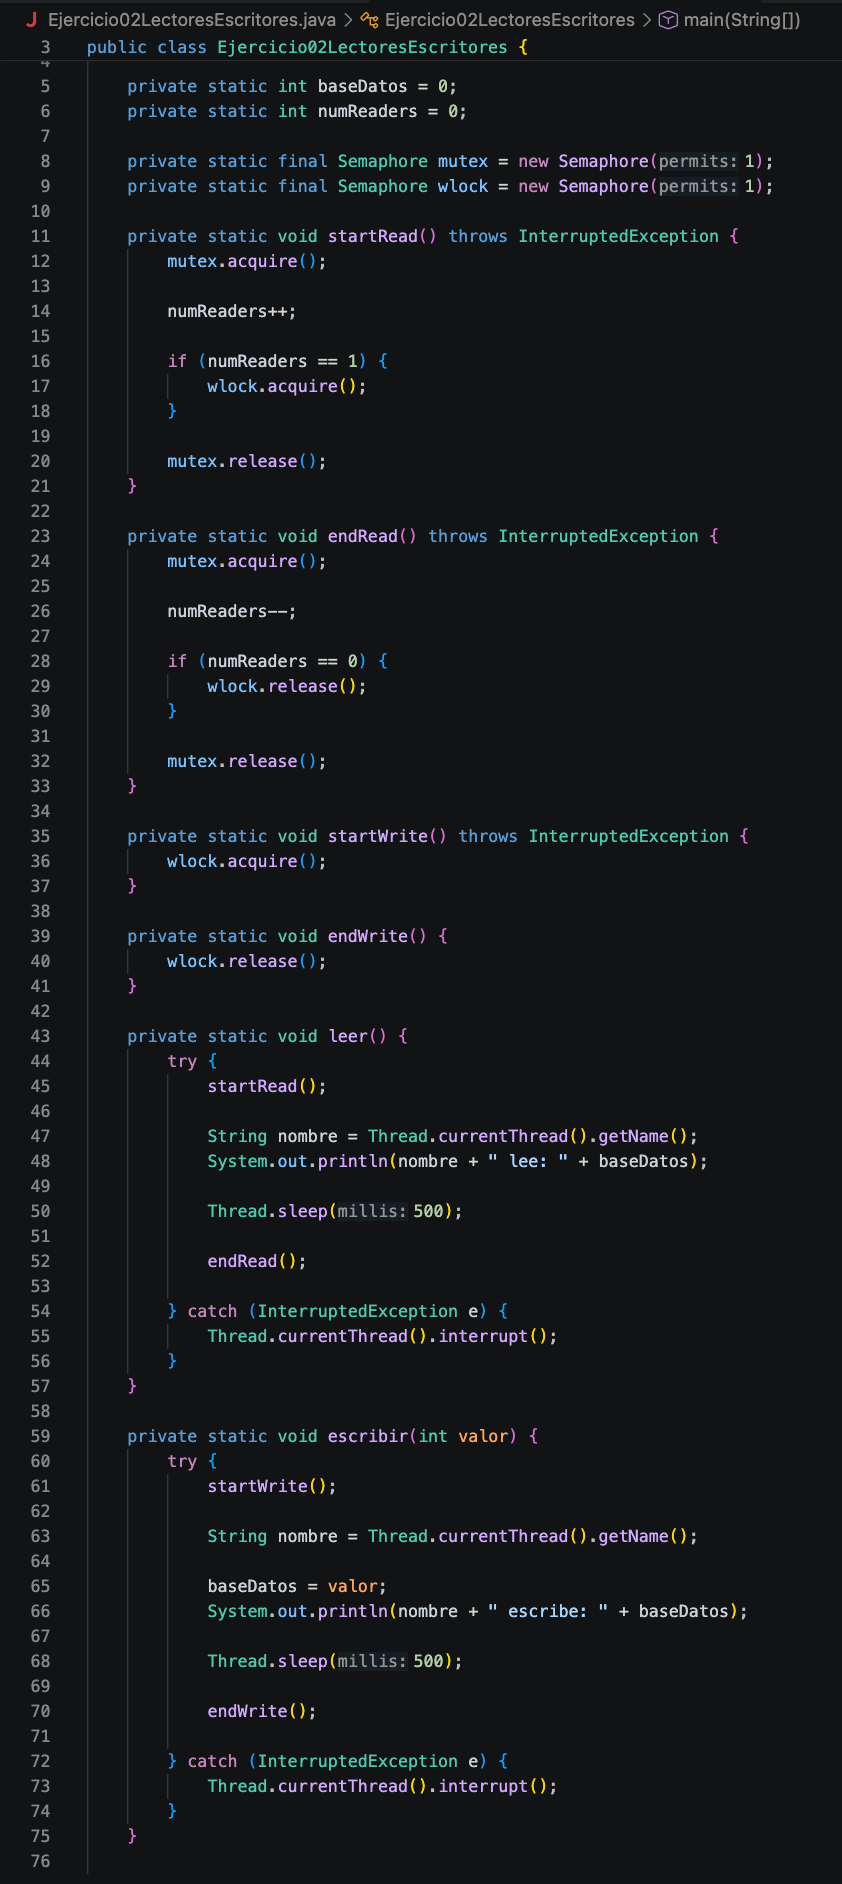
\includegraphics[
    width=0.95\textwidth,
    height=0.75\textheight,
    keepaspectratio,
    trim=0 400 0 0,
    clip
  ]{Captura de pantalla 2026-10-03 a la(s) 10.35.23 a.m..png}
  \caption{Código Java de los lectores y escritores, parte superior.}
  \label{fig:lectores-escritores-metodos-superior}
\end{figure}

\begin{figure}[H]
  \centering
  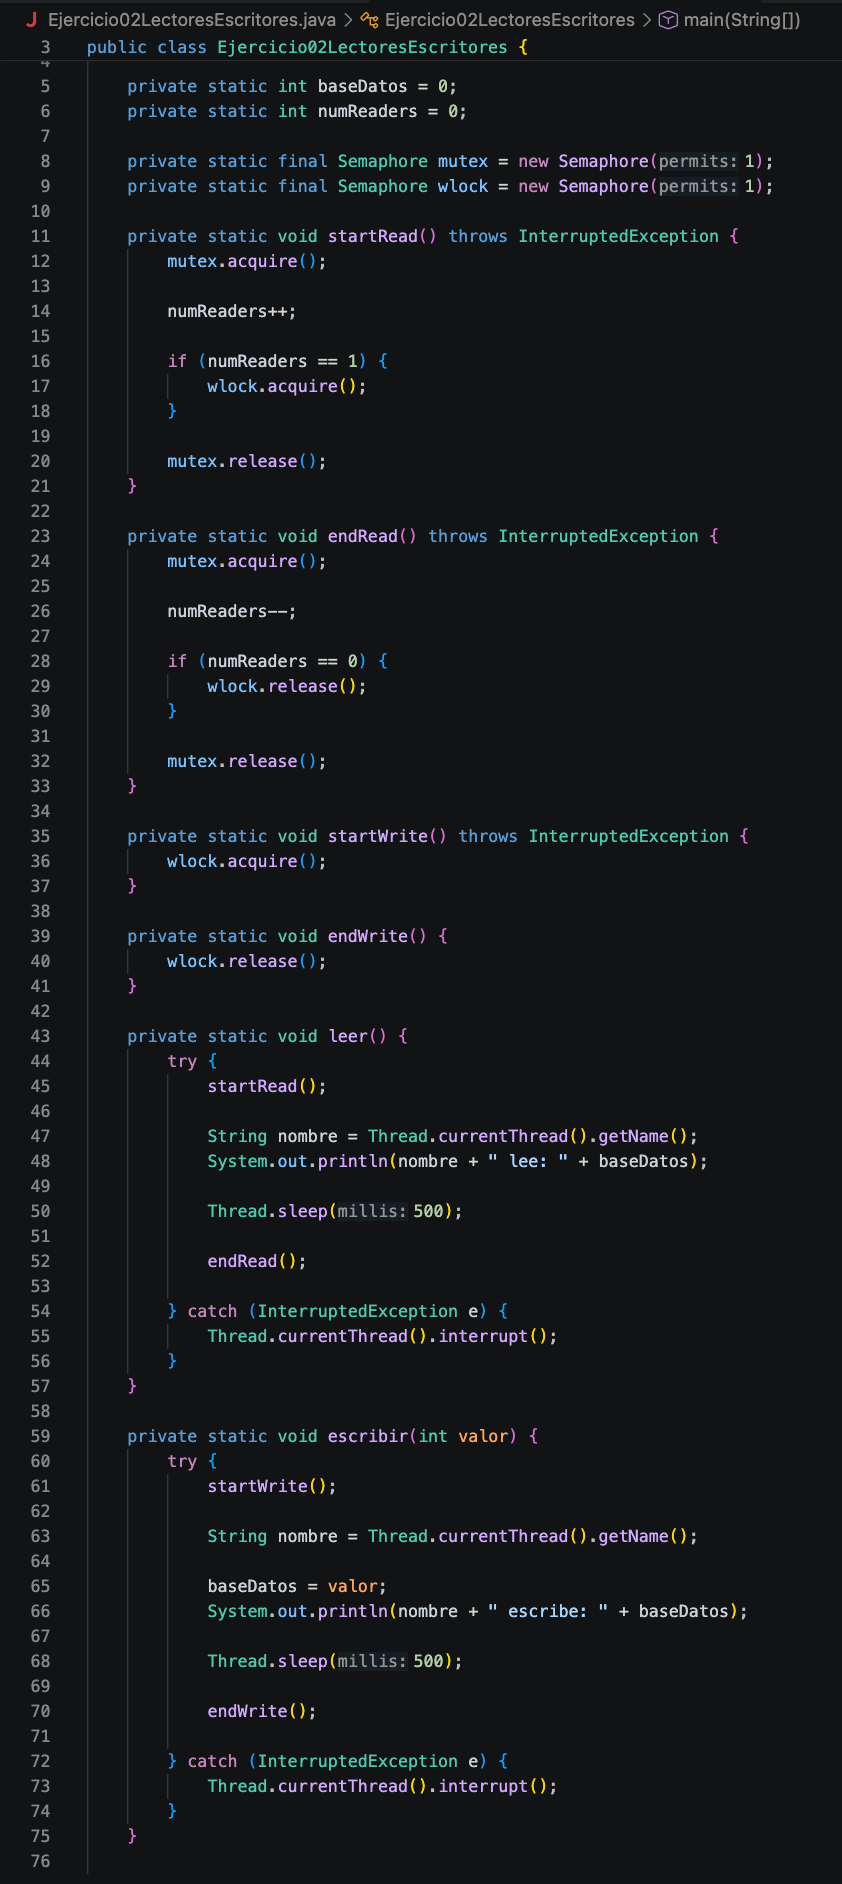
\includegraphics[
    width=0.95\textwidth,
    height=0.75\textheight,
    keepaspectratio,
    trim=0 0 0 480.75,
    clip
  ]{Captura de pantalla 2026-10-03 a la(s) 10.35.23 a.m..png}
  \caption{Código Java de los lectores y escritores, parte inferior.}
  \label{fig:lectores-escritores-metodos-inferior}
\end{figure}

\clearpage
\incluirevidencia[0.35\textheight]
  {Captura de pantalla 2026-10-03 a la(s) 10.35.00 a.m..png}
  {Creación de los hilos y resultados de las ejecuciones del problema lectores-escritores.}
  {fig:lectores-escritores-resultados}

\section{Conceptos utilizados}

En este problema, \texttt{mutex} protege una variable de control:
\texttt{numReaders}. El semáforo \texttt{wlock} protege la base de datos. La
exclusión mutua se observa cuando un escritor modifica la base de datos sin
que otro escritor o un lector pueda hacerlo al mismo tiempo.

La sincronización condicional aparece cuando un hilo debe esperar una
condición. Un escritor espera mientras exista al menos un lector. El primer
lector toma \texttt{wlock} y el último lector lo libera. Así, varios lectores
pueden compartir la lectura, pero las escrituras permanecen aisladas.

\chapter{Conclusión}

El problema productor-consumidor utiliza un semáforo binario y dos semáforos
contadores. El semáforo binario protege el búfer, mientras que los contadores
indican si el productor puede depositar o si el consumidor puede retirar. La
espera ocurre cuando el búfer está lleno o vacío.

El problema lectores-escritores utiliza un semáforo para proteger
\texttt{numReaders} y otro para controlar la base de datos. Los lectores
pueden entrar juntos, pero un escritor necesita acceso exclusivo. En ambos
programas los semáforos evitan condiciones de carrera y bloquean los hilos
solo cuando no se cumple la condición necesaria para continuar.

La exclusión mutua significa que una sección crítica solo puede ser utilizada
por un hilo a la vez. La sincronización condicional establece el momento en
que un hilo puede continuar, por ejemplo cuando aparece un espacio libre, un
elemento disponible o cuando termina el último lector.

\cleardoublepage
\phantomsection
\addcontentsline{toc}{chapter}{Referencias}
\nocite{*}
\bibliography{template/references}

\end{document}
